\documentclass[12pt]{report}
%\usepackage[utf8]{inputenc}
\usepackage{graphicx}
\graphicspath{ {images/} }
\usepackage{float}
\usepackage{indentfirst}
\usepackage{multirow}

\pagestyle{plain}
%\linespread{2}
\usepackage{setspace}
%\doublespaceing

\newcommand\MyBox[2]{
  \fbox{\lower0.75cm
    \vbox to 1.7cm{\vfil
      \hbox to 1.7cm{\hfil\parbox{1.4cm}{#1\\#2}\hfil}
      \vfil}%
  }%
}

\pagenumbering{Roman}

\author{D.Siegle}
\title{Cytochrome P450 Inhibitor Classification with Statistical Learning}
\date{February, 17 2015}

\begin{document}

% generate the title
\maketitle

\begin{doublespacing}
\chapter*{Abstract}
% Self reference and then abstract goes here.
SIEGLE, DANIEL E, M.S.
``Cytochrome P450 Inhibitor Classification with Statistical Learning (2015)'' Directed by Dr. Weifan Zheng, 53pp.
\vspace{1cm}


This project compares methods of Cytochrome P450 inhibitor prediction based on compound structures. CYPs are a natural first choice in which to  develop \textit{in silico} models because of their central role in drug candidate rejection due to adverse drug-drug interactions. Several non-linear, high-dimensional classification models were built and compared using a large, publicly available high throuhput screening luminescence assay (PubChem AID1851) against five CYP isozymes (1A2, 2C9, 2C19, 2D6 and 3A4). The methods compared are a Bayseian binary QSAR method from the Molecular Operating Environment, and 3 standard machine learning methods implemented in the Python programming language; $\kappa$-Nearest Neighbor, Random Forests, and Support Vector Machines. They all performed well, with the methods implemented in freely available software performing as well or better than the method in software that is widely accepted in industry. 
\end{doublespacing}

\tableofcontents
%\cleardoublepage
\addcontentsline{toc}{chapter}{\listfigurename}
\listoffigures
%\cleardoublepage
\addcontentsline{toc}{chapter}{\listtablename}
\listoftables

\begin{doublespacing}
\chapter*{Acknowledgements}
I want to thank ...

\pagenumbering{arabic}

\chapter{Background}

\section{Drug Discovery Productivity Challenges}

The goal of pharmaceutical sciences is to identify safe and efficacious drugs for the market. Toxicity is a large contributor to drug candidate attrition in drug development. Inhibition of enzymes in the cytochrome P450 superfamily is a major source of toxicity in human and animal models because of their role in first pass metabolism. If a compound inhibits cytochrome P450, toxic effects are likely to follow if first pass metabolism fails to clear other therapeutic compounds or alters their pharmacokinetics. Because the discovery and development of a each new pharamceutical drug requires more than a billion dollars across an average of 12 years, it would be useful to know whether a compound of interest inhibits cytochrome P450s as early as possible.

The Cytochrome P450 superfamily is large and varied. Different isozymes metabolize different substrates. Even within and between individuals pharmacokinetic and pharmacodynamic variability can be high for reasons not entirely characterized. Designing assays for every isozyme and single nucleotide polymorphic variant and running them against every compound of interest as a general strategy is cost prohibitive. This project was designed to test the predictive power of computational methods for cytochrome P450 inhibition potential based simply on knowledge of chemical structure.

There has been a downward trend in drug development productivity for the last three decades for a variety of reasons. The difficulty of improving upon current treatments in novel ways, increasingly cautious regulatory environments, and over-reliance on early stage identification of 'silver bullet' treatments that end up as late stage failures have all been suggested as causes of this productivity decline.  \cite{Scannell2012} Integrated computational approaches have been proposed as one way to control costs in ongoing pharamceutical research and development. \cite{Visser2014} The foundational skills demonstrated in this thesis are needed to pursue a systems approach to drug development that industry has recently turned toward as a way to boost R\&D productivity. \cite{Berg2014} This thesis is also part of the larger project of \textit{in silico} drug-development, which is attempting to reduce reliance on exploratory \textit{in vivo} and clinical drug testing and increase the number of effecive treatments for patients while decreasing the amount of time to develop them.

The Quantitative Structure Activity Relationship (QSAR) approach to associating compound structure with bioactivity that goes back at least to Hansch\\ \cite{Hansch1964}, has a long history with \textit{in silico} drug-development efforts. QSAR started with direct measures of chemical compounds and then later derived features, and used them to then build expert systems or statistical models that tried to predict biological activity. During those same decades, the field of machine learning emerged; using computation in an analogous and more general way -- to associate features with results, inputs with outputs. Machine learning can be thought of as using algorithms to figure out how to perform important tasks by generalizing from examples. These algorithms are of course usually laborious, which necessitates their execution by computer.

Statistical machine learning builds upon the peer prediction of machine learning. It also allows for prediction but focuses more on models and methods that can be used by scientists and engineers. \cite{James2013} Further extension of statistical learning to the pharmaceutical sciences can lead to important contributions to systems pharmacology. Or rather, statistical learning methods are an important precursor to the needs of systems biology and systems pharmacology modeling.

This project compares different techniques for cytochrome P450 inhibition prediction in the framework of statistical learning. In order to demonstrate generality and aplicability to the pharmaceutical sciences, the subjects of this study are the five isozymes of Cytochrome P450 (CYP) that are involved in metabolism of 90\% of all therapeutic drugs (CYPs 1A2, 2C9, 2C19, 2D6 and 3A4). \cite{Veith2009}

Because replicability is one of the main principles of the scientific method, as much as possible, the code and data used in this study is source controlled and publicly available. Reproducibility as a practice is a habit, and a good one to get into. Every attempt was made to make the materials and methods for this project reproducible in a completely automated way to allow for validation of results and extension of the work.

\section{Cytochrome P450 Superfamily}

One of the largest and most functionally diverse protein superfamilies is the cytochrome P450 family of hemoproteins. From bacteria to humans, the functional breadth of cytochrome P450 activity is far ranging. At the latest count there were significantly more than 2000 identified cytochrome P450 genomic and cDNA sequences that have been divided into a total of 265 different families. \cite{Danielson2002} Cytochromes P450 appear in every kingdom from bacteria to higher eukaryotes. Multiple cytochrome P450 genes can be expressed simultaneously as different isozymes and the number of genes per species is highly variable with a tendency for higher eukaryotes to possess more. The cytochromes P450  constitute the major enzyme family capable of catalyzing the oxidative biotransformation of most drugs and other lipophilic xenobiotics and are therefore of particular relevance for clinical pharmacology. The central role that these ubiquitous proteins play as phase I enzymes in human drug metabolism makes them very important to the pharmaceutical industry.

\begin{figure}[H]
  \centering
   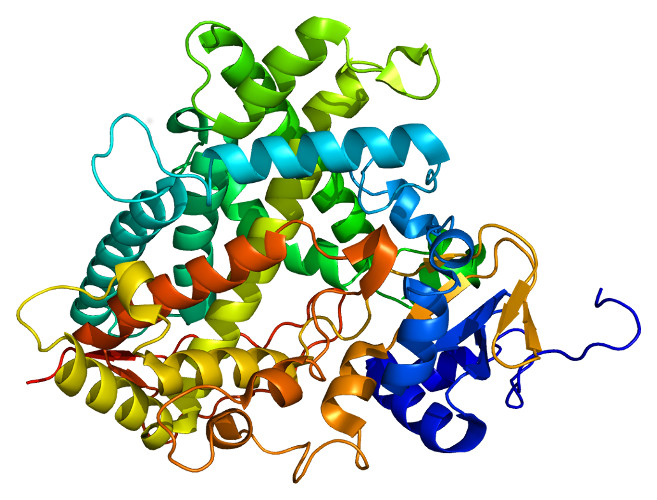
\includegraphics[width=1\textwidth]{../img/CYP1A2_PDB.jpg}
  \caption[Ribbon Diagram of CYP1A2]{Ribbon Diagram of CYP1A2 (PDB 2HI4)}
\end{figure}

CYP families are classified based on pairwise amino acid sequence identity between individual members. Families CYP 1-3 are involved in phase I metabolism of human drugs and xenobiotic compounds, whereas other CYP families (CYP 4, 11, 17, and 21) are involved in the metabolism of endogenous compounds such as fatty acids, steroids, eicosanoids, bile acids and fat soluble vitamins. \cite{Singh2011}

\begin{figure}[H]
  \centering
   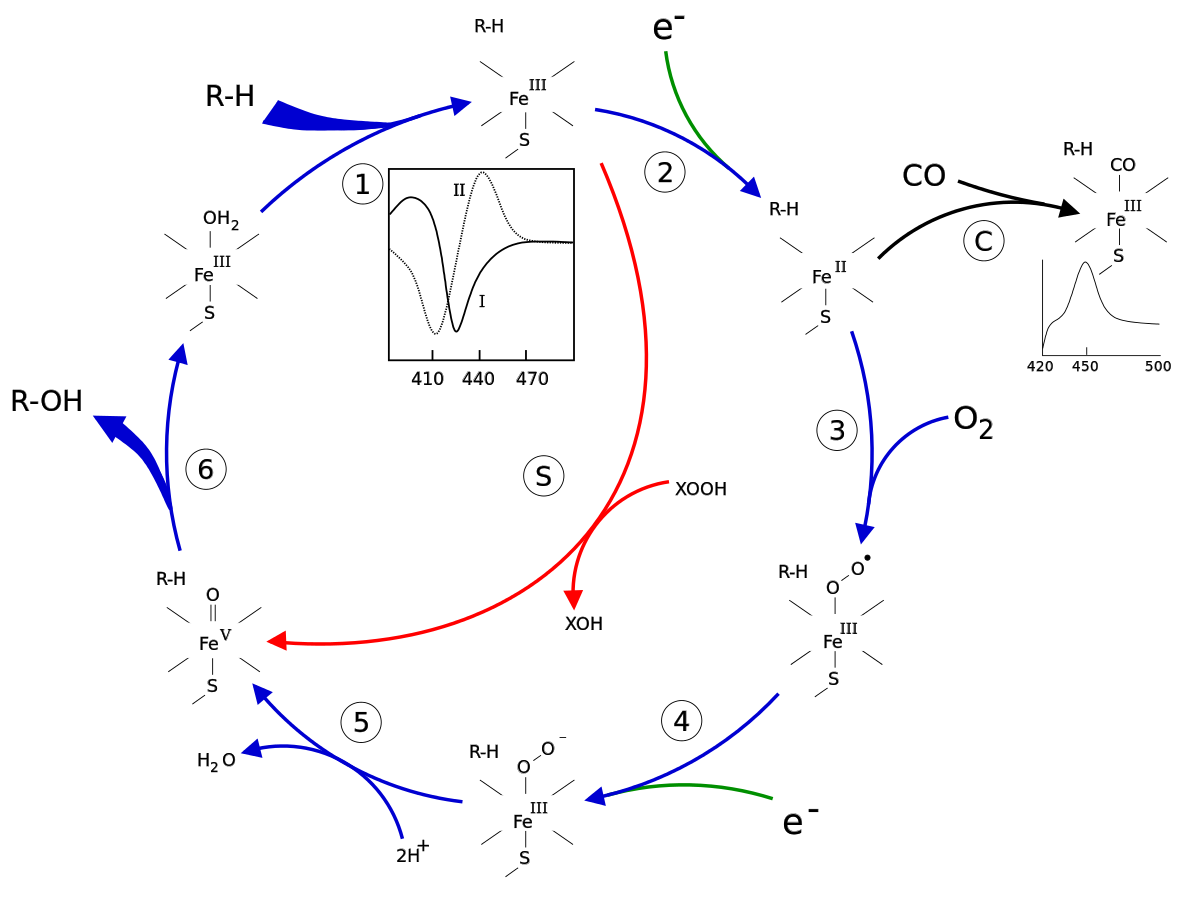
\includegraphics[width=1\textwidth]{../img/P450MOA.png}
  \caption{Mechanism of Action of Cytochrome P450 Catalytic Heme Group}
  \label{fig:P450MOA}
\end{figure}

Figure \ref{fig:P450MOA} illustrates the catalytic cycle that occurs at the central heme group in all Cytochromes P450 as follows:
\begin{enumerate}
\item First the substrate binds and induces a conformational change in the enzyme that usually displaces a water group. This brings the substrate in close proximity to the heme group.
\item Bound substrate induces electron transfer from a nearby reductase that provides NAD(P)H. At this point the -CO complexed with the heme group absorbs light spectra at max 450nm, noted by the 450 in the original naming of Cytochromes P450.
\item A second oxygen molecule displaces a carbon followed shortly by
\item A second electron transferred from a nearby reductase that leads to
\item Rapid double protonation of the peroxo group that results in one molecule of water being released, leaving the ferrous center with one double bound oxygen molecule. An alternative route this chemical state is shown by the S step in Figure \ref{fig:P450MOA}, called the 'peroxide shunt', that entails oxidation of the heme center directly.
\item At this point, it depends on the substrate and isozyme involved as to what sort of reaction is catalyzed, but the figure shows a hydroxylation, which is a very common way to make lipophilic substances more water soluble.
\end{enumerate}

\begin{figure}[H]
  \centering
   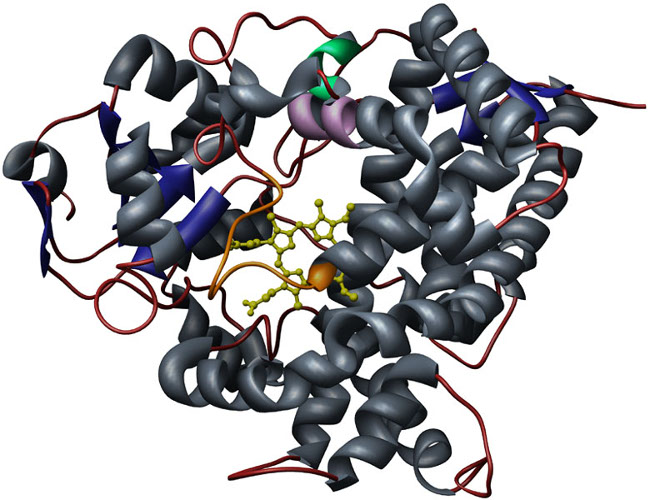
\includegraphics[width=1\textwidth]{../img/CYP3A4_heme.jpg}
  \caption[Ribbon Diagram of CYP3A4 with Heme Center]{Ribbon Diagram of CYP3A4 with Heme Center Highlighted (PDB 1W0E)}
  \label{fig:heme}
\end{figure}

There is a considerable substrate overlap between enzymes of this superfamily. Being broadly specific with respect to their substrates, CYPs are therefore susceptible to inhibition by a large variety of chemical compounds. It follows that the CYP enzymes that are involved in the oxidative metabolism of drugs play a major part in the activation and elimination of therapeutic drug molecules. CYP inhibition that leads to decreased elimination and/or changed metabolic pathways of other substrates is a major cause of adverse drug-drug interactions. \cite{Lapins2013} So adverse side effects of drug-drug interactions are an important area of inquiry, especially during the research phase of drug discovery.


\section{Early Compound Profiling \textit{In Silico}}

Drug discovery is a multi-parameter optimization process in which compounds are designed for interaction with their target while simultaneously minimizing off-target activities. \cite{Zlokarnik2005} In the normal course of taking a compound from hit to lead to drug candidate, adding drug-like properties may minimize the risk of making potent and target-class selective compounds that are biologically inaccessible, but at the same time does little to address the combinatorical complexities of specific drug-drug interactions due to off-target effects.

Because of the complex nature of toxicity, safety prediction is considered more challenging than efficacy prediction for a number of reasons. \cite{Kruhlak2012} Toxicity mechanisms may be unknown or poorly characterized in higher organisms, and similar pathways and targets may be associated with different toxicities and adverse events. Toxicity prediction must also encompass a number of complex interactions and remain alert to the possibility of finding the unexpected. For instance, toxicities could result from on-target effects due to incomplete knowledge or inadequate target validation, or from off-target effects mediated via unknown molecules and mechanisms, or even from genetic variation or comorbidities in any of the previously mentioned pathways.

Techniques for high-throughput \textit{in vitro} screening of CYP inhibition have been developed and implemented broadly in drug discovery pipelines across pharmaceutical companies and research institutions, resulting in the generation of large, varied sets of data. Some of this accumulation of data has been released through academic research initiatives (e.g. PubChem Bioassays AID 410 and 1851). These collections enable development of structure-activity relationship models for \textit{in silico} prediction of CYP inhibition by a much larger pool of researchers than those who designed and carried out the assays.

The promise of \textit{in silico} screening that remains very appealing is that, with a steady increase in computing power, screening costs could become negligible. The hope is that virtual compounds could be screened for CYP liabilities in order to realize savings and reduce the number of candidates with questionable prospects that would otherwise have to be synthesized. \cite{Zlokarnik2005} Achieving this would also turn the costly animal toxicity test phase of preclinical research into a validation step rather than a screening step.

In order to generate the necessary data, many high-throughput technologies are now available to detect P450 inhibitors. Combining high-throughput screening data from various assays can be used to guide medicinal chemists away from inhibitory interactions at an early stage. In certain cases it might also identify the inhibition issue allowing intervention by targeted modification of the CYP interacting functionality. According to Zlokarnik, to be generally useful, P450 inhibition screens need to be calibrated against standard methods and preferably also tested with a large set of drugs, for which human drug-drug interaction outcome is known. \cite{Zlokarnik2005} This should also decrease the number of withdrawls of novel drugs from the market due to inhibition of major P450 isozymes.

The ability to predict clinical safety based on chemical structures has recently become an increasingly important part of regulatory decision-making. QSAR models are currently used by in industry and by regulators to evaluate safety concerns and possible nonclinical effects of a drug when adequate safety data is absent or inconclusive. \cite{Kruhlak2012}

As an example, the United States of America is about to become the last country to accept QSAR in the drug approval process. The drafting of International Committee on Harmonization (ICH) M7 guideline can be viewed as setting a precedent for possible future, broader regulatory applications of QSAR modeling. ICH M7, will for the first time specify that -- under very specific conditions -- the results of QSAR computational toxicology predicitions will be considered sufficient for genotoxic contaminants of pharmaceuticals under consideration and thereby eliminate the need for laboratory testing. \cite{Kruhlak2012}


\section{Quantitative Structure-Activity Relationship}

Quantitative structure-activity realtionship modeling is generally accepted as the construction of predictive models of biological activities as a function of structural and molecular information of a compound or compound library. \cite{Nantasenamat2009}

QSAR models describe the correlation between molecular features and activity at a given end point of interest. There have also been attempts to make structure activity relationship (SAR) models constructed by using human expert knowledge (“expert rule-based”), but QSAR models are typically defined as those that use mathematical methods to analyze the statistical correlations between molecular features and activity. 

A QSAR model that defines the mathematical relationships between descriptors and biological activities of know molecules differs from receptor binding-based efficacy prediction which takes into account binding site characteristics as well as molecular docking analysis. In contrast to QSAR, receptor-binding methods attempt to predict drug efficacy based on known mechanisms of action and medicinal chemistry by individually studying molecular interactions between a drug and targets/receptors. \cite{Kruhlak2012}

It follows from the 'similarity principle' that new and untested compounds possessing similar molecular features to known compounds are assumed to possess similar activities and properties. In this way, QSAR models can make it possible to predict the biological activities of a given compound as a function of its molecular structure. Several successful models have been published over the years which encompass a wide spectrum of biological and physicochemical properties.

Applied QSAR, as described above, has typically been used for drug discovery and development but has also been used to correlate molecular information with other physiochemical properties. This later approach is termed quantitative structure-property relationship (QSPR). Derived molecular parameters can account for hydrophobicity, topology, electronic properties, and steric effects among other things. These characteristics of compounds can either be determined empirically through experimentation or theoretically via computational chemistry as needed. \cite{Nantasenamat2009} The parameters derived from compound structure are refered to as molecular descriptors.

\subsubsection{Molecular Descriptors}
Molecular descriptors can be thought of as the mathematical representation of essential information of a molecule in terms of its own physiochemical properties. Depending on the needs of the analysis, properties considered can be electronic, geometric, hydrophobic, constitutional, lipophilic, steric, solubility, quantum chemical, or topological. From a practical viewpoint, molecular descriptors are chemical information that is encoded within the molecular structures. \cite{Nantasenamat2009}

Molecular features can be either experimentally measured or calculated values. They come in the form of simple physiochemical properties such as logP or logarithmic acid dissociation constant (pKa), numerical representaions of substructure fragments, or purely mathematical descriptors. Mathematical descriptors are chemical structural features represented in numerical form, and range from simple atom counts to the product of complex equations that describe electron distribution across a molecule. \cite{Kruhlak2012}

Molecular descriptors as predictors in QSAR modeling are typically less precise than the “lock and key” relationships that underpin the docking approach to computer-aided drug design. The basic assumption in QSAR modeling is that similar molecules exhibit similar biological activity so that physiochemical properties and/or structural properties of a molecule encoded as molecular descriptors can then be used to predict the biological activity of structurally related compounds with some degree of confidence.

\subsubsection{Modeling}
QSAR models can be described as global or local. Global models incorporate chemicals with a range of molecular features acting across the spectrum of chemical pathways, whereas local models are highly focused on a single chemical class and end point. Although local models generally have much higher accuracy, their narrow domain of applicability renders them impractical in most regulatory environments where predictions need to be made across a variety of molecules including active pharmaceutical ingredients, as well as metabolites, reagents, and synthetic intermediates. \cite{Kruhlak2012} Therefore, the focus of this study is global model construction.

The construction of QSAR models typically consists of two main steps:
\begin{itemize}
\item Description of molecular structure with derivation of descriptors
\item Multivariate analysis correlating molecular descriptors with observed activities. 
\end{itemize}
Additional intermediate steps are also crucial for sucessful development of such QSAR models and include data preprocessing and statistical evaluation. See Figure \ref{fig:QSARworkflow} \cite{Nantasenamat2009}

\begin{figure}[h,t]
  \centering
  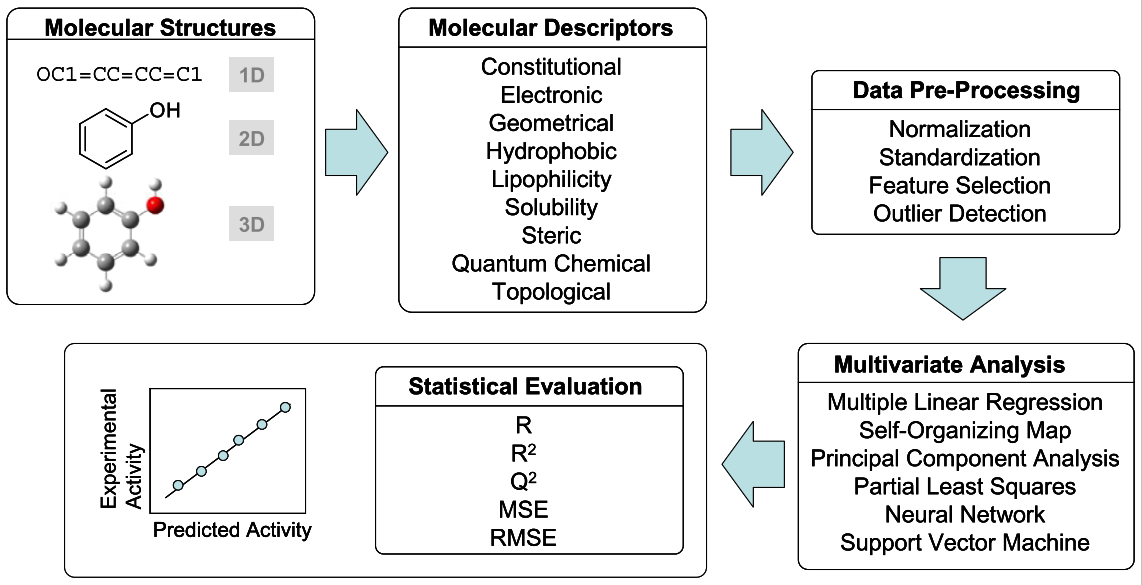
\includegraphics[width=1\textwidth]{../img/SchematicQSAR.png}
  \caption[Typical QSAR Workflow]{Typical QSAR Workflow \cite{Nantasenamat2009}}
  \label{fig:QSARworkflow}
\end{figure}

A typical QSAR workflow treats chemical structure management, descriptor calculation, and statistical analyses as separate steps that are often performed by non-integrated software packages. This can lead to low throughput and even the lack of possibility of performing predictions for new compounds or the inability to update the models when new data become available, depending on the workflow. Approaches that integrate as many of these steps as possible are generally preferred.

According to Kruhlak, et al., the successful development of a QSAR model for safety prediction requires a sufficient amount of high-quality data, the appropriate selection of descriptors, the availability of one or more suitable statistical or mathematical models and an effective training and validation strategy.
\cite{Kruhlak2012}

\section{Statistical Machine Learning}

Machine learning algorithms figure out how to perform important tasks by generalizing from examples. A concise definition of statistics is as the applied science that constructs and studies techniques for data analysis. (Jan de Leeuw) Statistical learning refers to a set of approaches for estimating a function that describes a dataset as a precursor for prediction or inference. \cite{James2013} Statistical machine learning constructs that function by generalizing from examples, i.e. data.

Leo Breiman wrote a landmark paper that documented the beginnings of this approach. He said 
\begin{quote}
'There are two cultures in the use of statistical modeling to reach conclusions from data. One assumes that the data are generated by a given stochastic data model. The other uses algorithmic models and treats the data mechanisms as unknown' \cite{Breiman2001}
\end{quote} He goes on to claim that the statistical community had traditionally prefered the first view.

Classification is a well understood area of machine learning. A classifier takes a system of inputs, typically a vector of discrete and/or continuous feature values and then outputs a single discrete value, the class. \cite{Domingos2012} It can be used when there are multiple examples of items of interest that are then used to guide the identity determination of a new item based on its characteristics.

The current state of machine learning is fundamentally a subset of optimization and has found its biggest successes in fields where there are far more variables than parameters. The ultimate goal of machine learning in these cases is to generalize beyond examples in a training set, because no matter how many examples the training set contains, it is unlikely that those exact examples will be seen again in practical applications. \cite{Domingos2012} 

In the context of QSAR then, with enough prior knowledge and sound assay results, machine learning may be a practical approach to fill in the gaps of clinical knowledge for any relevant CYP isozyme when queried against any untested compound of interest so long as the compound structure is known.

This is a wider view than traditionally encountered in most applied science education where simple hypothesis testing predominates. Opening up the field of drug discovery to data analysis like this brings opportunity for exploration but also new concerns, such as the 'curse of dimensionality', 'degrees of freedom of the analyst', 'black box algorithms', bias estimation difficulties and the 'no free lunch theorem'. \cite{Boulesteix2014}

\section{Sources of Data for Learning}

Systems biology research encompasses the generation of high-throughput datasets of system components (omics data), experimental methods of analysis and data integration, as well as the development and application of network approaches and computationally derived models. In pharmaceutical research, systems biology efforts are directed towards the identification of drug targets, the development of novel therapeutics and new indications for existing drugs. \cite{Berg2014}

Omics tools, developed over the past several decades, can provide global information on the levels and dynamic changes in cellular and tissue components at specific time points in samples from cell-based assays, precinical animal models and human studies. Omics data sets derived from transcriptomics, proteomics, and metabolomics can also be used and integrated with each other, as well as with genomics information and other data types, to construct models of cell signaling, pathway and disease networks. These models may help to identify new targets as well as better understand and predict drug action \textit{in vivo}.

\begin{quote}
The ultimate goal of systems biology in this context is an understanding of physiology and disease across the multiple hierarchical levels of organization, from chemical and molecular interactions to pathways and pathway networks, at the cell-cell and tissue level, organs and organ systems and, ultimately, to the functioning of the whole organism. \cite{Berg2014}
\end{quote}

The data available for learning in discovery and development of pharmaceuticals tends to be compound-centric. Compound data collections are generally concerned with the identification and characterization of small molecules or biologics that selectively inhibit (or activate) specific molecular targets or pathway mechanisms. These kinds of studies are particularly useful to drug discovery research as the attempt to work out related drug mechanisms of action. These studies also inform secondary drug development goals, such as clinical indication selection and patient stratification. \cite{Berg2014}


\section{Reproducibility}

Several recent publications have highlighted the negative impact of irreproducible biomedical research, such as the group from Bayer that claimed they had to halt two-thirds of their research efforts in 2011 \cite{Prinz2011} and the group from Amgen that reported only an 11\% success rate in trying to replicate the effects of major cancer drug findings. \cite{Begley2012} In the latter case we don't even know which drugs were tested because those findings are not public either. Information generation can happen far faster and is much more common than data analysis and knowledge creation in the biological sciences.

Some of the issues to overcome in this area include the need for more biologists trained in quantitative and statistical methods for analyzing large data sets and the open release of findings and experimental protocols. 

Science conducted in an open fashion confers the following benefits

\begin{itemize}

\item Reproducibility of experimentation allows other researchers to use the exact methods to calculate the relations between biological data.

\item Faster development of disease models and therapeutic treatments due to the reuse of existing knowledge. Projects can be built upon existing results more easily or used to extend the research in directions unanticipated by the original team. First-pass results can be subject to new analysis and a second look at compounds with interesting side effects can lead to serendipidous discoveries.

\item Increased quality as a result of having more researchers studying the same topic to provide a layer of assurance that errors will not propagate.

\item Long-term availability of data and code. If these resources are not tied to businesses or patents, then they can be posted to multiple repositories to ensure that they are available in the future.
\cite{Prlic2012}

\end{itemize}

New research findings, supporting data and methods should, therefore, be made publicly available for independent verification and replication in order not to delay medical advances.

\pagebreak

\section{Aims}
The aim of this project is to build QSAR models that quantify the risk of off-target effects for candidate molecules by building statistical machine learning models that make binary classification as inhibitors or non-inhibitors of Cytochrome P450 of compounds based on their structure.

We will compare a well accepted, commercial method of binary classification with three open source implementations of QSAR model building according to the following plan:

\begin{itemize}

\item Build Binary QSAR models in the Molecular Operating Environment (MOE).

\item Develop and implement comparable methods in open source software.

\item Evaluate and compare results from all models.

\item Perform this analysis as reproducible research.

\end{itemize}


\chapter{Materials and Methods}



\section{Review of PubChem Assay 1851}
  

PubChem BioAssay 1851 contains data for inhibition of five major CYP isoforms (1A2, 2C9, 2C19, 2D6 and 3A4) by 17,143 chemical compounds. \cite{Veith2009} The the tested compounds were all drugs or drug-like compounds. The chemical space revealed that the majority of compounds had molecular weight below 500 daltons and logP below 5. \cite{Lapins2013}

The assay used low low-fluorescence substrates, which are converted to more-fluorescent metabolites. The progression of the reaction is measured by an increase in fluorescence intensity during CYP isozyme metabolism of the substrate. Inhibitors of a particular CYP reduce the rate of metabolism of the substrate and this results in a decreased fluorescence signal. \cite{Zlokarnik2005}

The most recent technology developed for CYP inhibition is based on substrates that release luciferin as the metabolite. This is a coupled assay system in which addition of luciferase and ATP converts the freed luciferin to des-carboxyluciferin with light emission. The format is similar to fluoresence methods, and all that is required is addition-only manipulations and luminescence plate readers. \cite{Zlokarnik2005} The assay obtained lumiescence readings at a range of compound concentrations and then determined activity parameters using the Hill equation.


%Inorganic compounds, non-covalent inhibitors and compound mixtures were removed from the dataset, leaving 16,359 compounds. \cite{Lapins2013}

In the dataset, compounds are classified as active or inactive inhibitors for each CYP with an activity cutoff set to AC50 = 10uM (AC50, “activity concentration 50”, refers to the concentration that is required to elicit half-maximal effect). However, in cases where the dose-response curve for a compound showed poor fit or the inhibition efficacy was below 60\%, the assay results were regarded as inconclusive. \cite{Lapins2013}

Compounds were characterized by their Activity Score and regarded as inhibitors if their activity score ranged between 40 and 100. PubChem Acitivity Score is assigned based on AC50 value, which was combined with a confidence measure. Combining measures for completeness of a dose-response curve and efficacy of inhibition, resulted in the Activity Score, where a larger value indicates higher inhibitory activity and/or higher confidence in inhibitory assay result. Compounds with an activity score equal to zero are considered as non-inhibitors while compounds with activity scores above 0 and up to 40 are considered inconclusive. \cite{Lapins2013}

The data from Pubchem Assay 1851 is available for download from the NIH through the PubChem website. The interface changes from time to time, but I downloaded two files which comprised the entire dataset for the experiment. The first file, a structures file, contained the structural information encoded in the simplified molecular-input line-entry system (SMILES) format for each tested compound with corresponding Structure ID (SID) and Compound ID (CID) as assigned by NCBI. Another file, also organized by SID and CID, contained all of the luminescent responses from the high-throughput screen and the fitted parameters which are then summarized by the activity score. 

\begin{figure}[!htbp]
  \caption{Supervised Learning Scheme for Clasification}
  \centering
  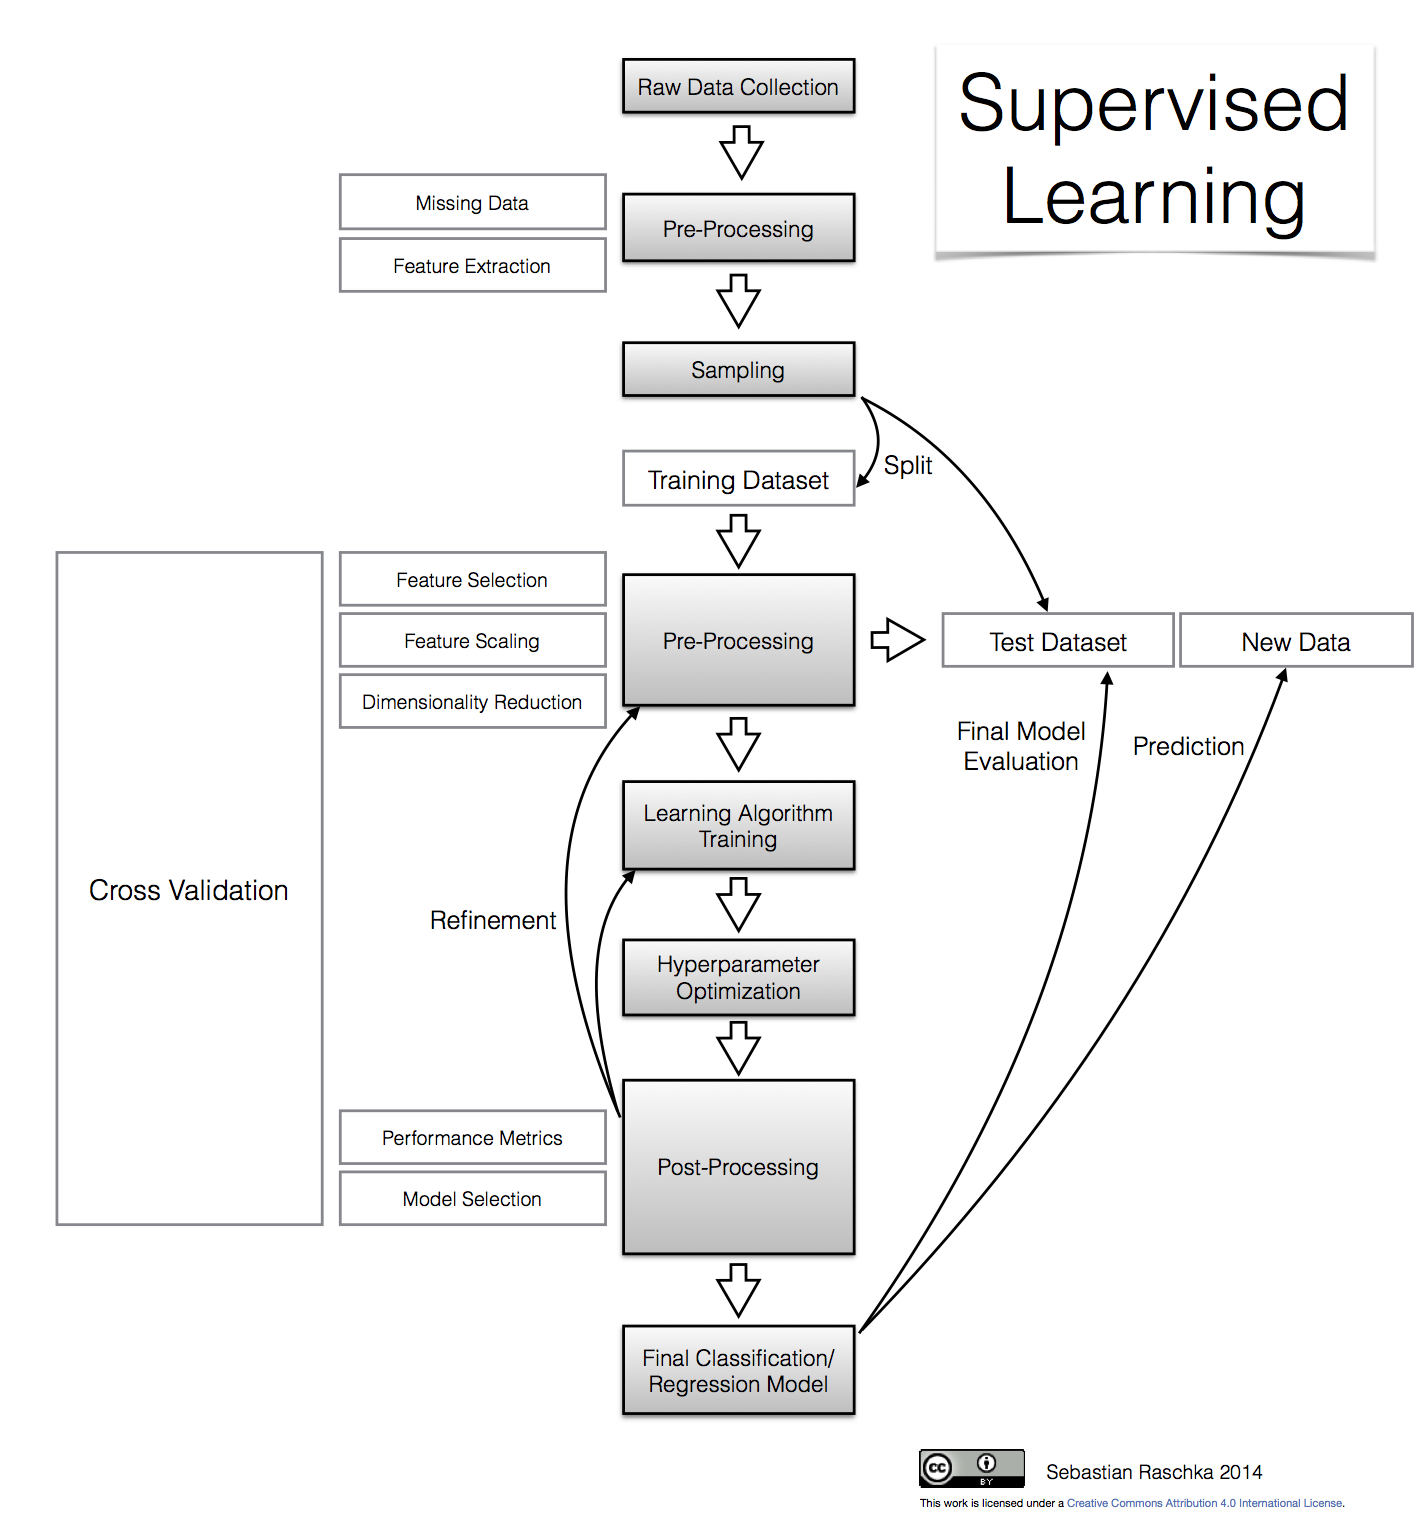
\includegraphics[width=1\textwidth]{../img/supervised_learning_flowchart.png}
\end{figure}


\section{Data Set Preparation and Molecular Descriptor Generation }

Both data files from Bioassy 1851 were downloaded as comma separated value (.csv) files and merged together based on the SID column using functions from Python's pandas library, which is made for handling, manipulating and reshaping structured data.

The preliminary steps of data preprocessing typically requires data cleaning as raw data often contain anomalies, errors, or inconsistencies such as missing data, incomplete data, and invalid character values which may cause trouble in data analysis if left untreated. It is more complicated when data are collated from many formats that require harmonization and redundancy elimination. \cite{Nantasenamat2009} In this case, minimal preprocessing was required due to the polished nature of the source files.


\begin{figure}[h,t]
  \caption{Data download and preparation}
  \centering
   \includegraphics[width=1\textwidth]{}
\end{figure}


\subsubsection{Molecular Descriptor Generation}
First the merged file was loaded into a database in the Molecular Operating Environment. MOE functionality was used to obtain the washed configuration of compounds by removing the salts and finding an energy-minimized conformation. MOE was then used to calculate descriptors based on the molecular structures. The entire suite of MOE 2-D descriptors was selected for descriptor generation, resulting in 186 additional columns of nominal, ordinal and continuous vales appended to the database. The resulting master file was saved in .csv format.

The dataset was then split by isozyme into 5 separate files that each contained only the SID, the Activity Score, and the 186 MOE 2-D descriptors using a script in the Python programming language.

For each isozyme, the number of active inhibitors was far outnumbered by the number of inactive inhibitors. The data file for each isozyme was subjected to a Python script that separated the inactives from actives. Then the order of the inactives was randomly shuffled and the column trimmed to the length of the activity column, thereby balancing the number of inactives and actives as required by some of the later statistical analyses. 

\begin{figure}[h,t]
  \caption{Isozyme data set preparation}
  \centering
   \includegraphics[width=1\textwidth]{}
\end{figure}

Next the script randomly shuffled the balanced datasets and split them into a training set and a test set. The training set held 80\% of the original values and the test set held 20\% of the original values. The split was not based on activity score. The ratio of active/inactive in each split was inspected to check if they were still acceptably balanced.

For each use of randomness in computation, a seed number was set for the random number generator to ensure reproducible results.  

The balanced and split datasets are saved to Figshare.com for permanent, free and open access. (http://dx.doi.org/10.6084/m9.figshare.1181846 and http://dx.doi.org/10.6084/m9.figshare.1066108) All subsequent analyses use these same splits for comparability.

\section{Feature selection}

Typically data sets often contain redundant or noisy variables which make it more difficult for learning algorithms to discern meaningful patterns from the input. Such multicollinearity of the variables can either be used or treated if necessary to reduce computational resources required for model construction. \cite{Nantasenamat2009}

There existed a great deal of variability in the range and distribution of each variable in the data set. This can pose problems for algorithms using distance measurements in the learning step. These situations are handled by applying statistical techniques such as min-max normalization or z-score standardiation. 

In min-max normalization, the minimum and maximum value of each variable is adjusted to a uniform range between 0 and 1 according to the following equation: $ X_{norm} = \frac{X - X_{min}}{X_{max} - X_{min}}  $ In z-score standardization, essentially the variable of interest is subjected to statistical operation to achieve mean center and unit variance according to the following formula: $ z = \frac{x - \mu}{\sigma}  $ \cite{Nantasenamat2009}

In situations where the data does not have a Gaussian (normal) distribution, simple mathematical functions can be applied to achieve normality or symmetry in the data distribution. A commonly used approach is to apply logarithmic transformation on the the variable of interest in order to achieve distribution approaching normality. This is typically performed on dependent variables such as the modeled biological/chemical properties of interest whereby IC50 may be transformed to logIC50 or -logIC50. Practically, such mathematical operation is applied to each individual value of a given variable of interest. \cite{Nantasenamat2009}

\section{Modeling - Mapping Descriptors to Activity Data}

At this point a complete dataset is assembled for each isozyme that is balanced for the number of active and inactive inhibitors, and that dataset has been further subdivided into a traing set and a test set. The following section describes the different methods of feature selection, normalization and classification algorithms used in this study.

\begin{figure}[h,t]
  \caption{Supervised Classification Model Training and Validation Workflow}
  \centering
   \includegraphics[width=1\textwidth]{}
\end{figure}

\subsection{Binary QSAR in the Molecular Operating Environment}
PLS regression is a qunatitative method available in the Molecular Operating Environment that has shown poor predictive accuracy with this dataset as demonstrated by previous attempts in Dr. Zheng's lab.

The Binary QSAR approach outlined by Labute \cite{Labute1999} and included in the 2011 version of MOE, takes a Bayesian and probabilistic approach to classification of activity after reducing all the descriptors to principal components.

To carry out this analysis, first the training data was loaded into MOE and used a menu driven interface to initiate the Binary QSAR methods. A threshold value of 39 was selected; all activity values 40 and above will be considered active and all values 39 and below are considered inactive. The smoothing parameter was left at the default value of 0.25. MOE automatically performs principal component analysis on high-dimensional datasets before Binary QSAR and there was no way to use the fuul suite of molecular descriptors.

For each isozyme a number of models were built, each using a different number of principal components.  Each principal component is orthogonal and uncorrelated to the rest, and each one captures a portion of the total variance inherent in the dataset. The assumption is that inclusion of more principal components leads to more of the variance being accounted for in a classification decision. However, since each principal component is a linear combination of all the variables, the benefits of dimensionality reduction comes at the cost of interpretability.  For exploratory purposes, models with 2, 5, 10, 15, 20, 30, and 44 principal components were constructed. 

MOE models were written to .fit files and the model report saved as a .txt file.

\subsection{$\kappa$-Nearest Neighbor ($\kappa$NN}
The kNN algorithm predicts the class of a test set object based on the class membership of its $\kappa$ most similar training set objects. \cite{Lapins2013}

\subsection{Random Forest (RF)}
Random Forest is a classifier that consists of multiple decision trees. A decision tree is made of nodes and branches. At each node the dataset is split based on the value of some attribute that is selected so that the instances of different classes are predominately moved to different branches. Classification starts at the root node and is performed by passing the instances along the tree to leaf nodes. \cite{Lapins2013}

To introduce diversity between the trees of a random forest, a small subset of all attributes is randomly selected to take decisions at each node of each tree. The classification decision is performed by considering results of all trees by majority vote. The optimal size of the forest and the number of attributes to consider at each node were found by performing five-fold cross-validation. \cite{Lapins2013}

\subsection{Support Vector Machines (SVM)}
SVM is a machine learning technique for classification or regression that uses linear or non-linear kernel-functions to project the data into a high-dimensional feature space. \cite{Lapins2013}

%Correlation is performed in this hyperspace based on the structural risk minimization principle i.e., aiming to increase the generalization ability of a model. \cite{Lapins2013}

They applied the commonly used Gaussian radial basis function kernel optimal gamma (width of the kernel function) and error penalty parameter C were found after performing grid search on five­fold cross validation. \cite{Lapins2013}


\section{Model Evaluation and Validation}

The building blocks of a successful QSAR model are the accuracy of the input data, selection of appropriate descriptors and statistical tools, and most importantly validation of the developed model. Validation is the process where reliability and relevance of a procedure are established for a predetermined purpose. For QSAR models validation should target robustness, predicition performances and applicability domain (AD) of the models. \cite{Lapins2013}

Statistical evaluation in QSAR modeling is essential to validate the model as well as to evaluate its predictive performance. The predictive performance of a data set can be assessed by dividing it into a training set and a testing set. The training set is used for constructing a model and then the predictive performance of that model is evaluated on the testing set. Internal performance is typically assessed from the predictive performance of the training set while external performance can be assessed from the predictive performance of the independent test set that has never been seen by the training model. A commonly used approach for internal validation is known as N-fold cross-validation where a data set is partitioned into N number of folds. For example, in a 5-fold cross-validation 1 fold is left out as a testing set while the remaining 9 folds are used as the training set for model construction and then validated with that fold left out. In situations where the number of samples is limited, leave-one-out cross-validation is the preferred approach. In that case, the number of folds is equal to the number of samples present in the data set. \cite{Nantasenamat2009}

%Some standard measures of performance used for QSAR models are sensitivity, specificity, positive predictivity, negative predictivity and concordance. Additional measures such as the Matthews coefficient can be used as a single metric for comparing one model to another while correcting for bias. Because most stat models can be modified to have greater specificity vs sensitivity (or vice versa) by adjusting the training set or applying predictive filters, the Matthews coefficient can be used to determine when the modification is so extreme that it leads to overall degradation of the models’ performance.\cite{Kruhlak2012}

%Statistical parameters - Pearson's correlation coefficient (r) is a commonly used parameter to describe the degree of association between two variables of interest. Calculated r values have values between -1 and +1 which indicate direct (positive) and indirect (negative) correlation. For describing the relative predictive performance of a QSAR model, r is used to measure the correlation between experimental (x) and predicted (y) values of interest in order to observe the variability that exists between variables. This is calculated according to the following equation: ...

%Root mean squared error (RMS) is another commonly used parameter for assessing the relative error of the QSAR model. RMS is computed according to the following formula: ...

%F-test -- The statistical significance of QSAR models are typically assessed by performing an ANOVA and observing the calculated F values, which is essentially the ratio between the explained and unexplained variance. Comparison between multiple QSAR models can be performed when all models have the same number of degrees of freedom meaning that the same sets of compounds and descriptors are used. Each model yields a calculated F value and the best performing model is identified as those bearing the highest value.\cite{Nantasenamat2009}

%Degrees of freedom take into consideration the number of compounds and the number of independent variables that are present in the data set. This can be calculated using the equation n - k - 1 where n = \# of compounds k = \# of descriptors. The higher the value, the more reliable the QSAR model is. \cite{Nantasenamat2009}

%Mathematically speaking, an outlier is essentially a data point which has a high standard residual in absolute value when compared to other samples in the data set. A commonly used approach for detecting outliers is performed by calculating the standard residuals of all compounds in the data set of a QSAR model. \cite{Nantasenamat2009}

In model building, 5-fold cross validation was used in conjuction with model building on the training set for all of the models built in Python. After the test set was evaluated, two statistical metrics were used to the overall prediction accuracy and the True Positive and True Negative Rate. We assessed the predictive ability of the models by performing cross-validation and external predictions.

\subsubsection{Confusion Matrix}

A confusion matrix (or error matrix or table of confusion) is a representational summary of the performance of a classifier. All data points used in model building are apportioned along one axis according to their actual class value, and along another axis according to the value predicted by that model. For binary classification this results in a square matrix with two 2 columns and 2 rows.

\begin{tabular}{c >{\bfseries}r @{\hspace{0.7em}}c @{\hspace{0.4em}}c @{\hspace{0.7em}}l}
  \multirow{10}{*}{\parbox{1.1cm}{\bfseries\raggedleft Actual\\ Class}} & 
    & \multicolumn{2}{c}{\bfseries Prediction Class} & \\
  & & \bfseries p & \bfseries n &                     \\
  & p$'$ & \MyBox{True}{Positive} & \MyBox{False}{Negative} & \\[2.4em]
  & n$'$ & \MyBox{False}{Positive} & \MyBox{True}{Negative} & \\
  &  &  &  &
\end{tabular}

In this study, results that are both actual inhibitors according to assay data and predicted inhibitors according to the model results are deemed True Positives (TP). Similarly, actual noninhibitors that are predicted to be so are called True Negatives (TN). In the case of actual inhibitors predicted to be noninhibitors, these are labelled False Negatives (FN) and are the result of Type I errors. Noninhibitors classified as inhibitors by the model are refered to as False Positives (FP) and are the result of Type II errors.

\subsubsection{Accuracy}

The accuracy metric provides general information about how many compounds are misclassified. Accuracy is simply the percentage of correctly classified instances over the total number of instances and is calculated as
$$ ACC =\frac{(TP + TN)}{(TP + FP + TN + FN)} $$
where TP is the number of true positives, TN is the number of true negatives, FP is the number of false positives or over-predictions, and FN is the number of false negatives or missed predictions.

Accuracy is not an optimal measure of model performance if the data set is unbalanced (i.e. sizes of the classes are unequal) or if certain errors are to be considered more serious than others (e.g. false negatives compared to false positives). \cite{Lapins2013} For this reason, all datasets were rebalanced to contain roughly equal numbers of active and inactive inhibitors.

As a futher interogation of results, the true positive rate and the true negative rate are also calculated for all models. The true positive rate is the fraction of true positives out of all actual inhibitors and it is calculated as follows 
$$ True Positive Rate = \frac{TP}{(TP + FN)} $$
The true positive rate is also refered to as Sensitivity and in to MOE software it is called Accuracy on Active.

The true negative rate is the fraction of true negatives over the number of actual noninhibitors and is calculated as :
$$ True Negative Rate =\frac{ TN }{(TN + FP)} $$
The true negative rate is also know as the Specificity of a classification, and in MOE it is called Accuray on Inactives.

%\subsubsection{AUROC}
%In contrast to accuracy, the AUROC is a measure of discriminatory power that is insensitive to changes in class distribution and the costs of making certain errors. A ROC curve is obtained by calculating sensitivity and specificity at various discrimination threshold levels.

%Sensitivity is the fraction of true positives among all positively classified instances (the true positive rate) and is calculated as : 
%$$ sensitivity = \frac{TP}{(TP + FN)} $$

%Specificity is the true negative rate and is calculated as:
%$$ specificity =\frac{ TN }{(TN + FP)} $$

%An increased sensitivity is always accompanied by decrease specificity. A ROC curve is plotted as $sensitivity$ versus $1-specificity$, at varied discrimination cut-offs. An area under the ROC curve (AUROC) close to 1 means that the classifier can perfectly separate the two classes, whereas an area 0.5 indicated that the classifier performs no better than random guessing.\cite{Lapins2013}


\begin{figure}[h,t]
  \caption{General Data Analysis Workflow}
  \centering
   \includegraphics[width=1\textwidth]{}
\end{figure}

\subsubsection{Binary QSAR after PLS of descriptors}
The test sets were loaded and the washed structures were appended to the .csv files. All models were evaluated using the menu driven workflow in MOE and the classification probabilities were appended to the database file and saved as a .csv.  

The resulting file was loaded into a MS Excel spreadsheet and the predictions classified as actives or inactives. Predicted probabilities of $\geq$ 0.5 were evaluated as active inhibitor predictions. Confusion matrices were then tabulated within the spreadsheet for predicted vs actual actives and inactives. And from the confusion matrices accuracy scores were calculated - total accuracy, TPR, and TNR. These results were saved and the results reported below.

\subsubsection{Modeling in Python}
The Python programming language is a dynamically-typed, object-oriented interpreted language. Its primary strength lies in the ease with which it allows a programmer to rapidly prototype a project, although it also has a powerful and mature set of standard libraries that can facilitate large-scale production-level software engineering projects as well. Python has a very shallow learning curve and excellent online learning resources. The following amachine learning algorithms used in this study were used as implemented in Python's scikit-learn package.

\subsubsection{$\kappa$-NN Utilizing the Full Set of 2-D Descriptors}
The full models follow a similar procedure to the previous workflow, except they omit data reduction by principal component analysis and use the full descriptor set to consruct and evaluate models. 

For each isozyme separately, training data is loaded into a dataframe. The Activity Score is assigned the role of response variable and all 186 descriptors are identified as predictor variables. Predictor variables are scaled and normed to mean $0$ and standard deviation of $1$. kNN.fit method is called from the scikit-learn library to train a model, which then reports the confusion matrix and an accuracy score for the training model by five-fold cross-validation. TPR and TNR are calculated from the confusion matrix.

\subsubsection{Random Forest Classification Utilizing the Full Set of 2-D Descriptors}
For each isozyme separately, training data is loaded into a dataframe. The Activity Score is assigned the role of response variable and all 186 descriptors are identified as predictor variables. Predictor variables are scaled and normed to mean $0$ and standard deviation of $1$. RF.fit method is called from the scikit-learn library to train a model, which then reports the confusion matrix and an accuracy score for the training model by five-fold cross-validation. TPR and TNR are calculated from the confusion matrix.

\subsubsection{Support Vector Machine classification utilizing the full set of 2-D descriptors}
For each isozyme separately, training data is loaded into a dataframe. The Activity Score is assigned the role of response variable and all 186  descriptors are identified as predictor variables. Predictor variables are scaled and normed to mean $0$ and standard deviation of $1$. SVM.fit method is called from the scikit-learn library to train a model, which then reports a the confusion matrix and an accuracy score for the training model by five-fold cross-validation. TPR and TNR are calculated from the confusion matrix.

A script was written for each isozyme that performed these three fit methods in series. Code and results are documented in IPython notebooks that are currently hosted on github.com and freely accessible and downloadable. Presented in this way, they are more easily verifyable and extendable. Experimenting with other classification algorithms in scikit-learn simply requires adding new method.fit calls to the model building loop, because of the simple and consistent design of the scikit-learn library.



\chapter{Results}



Here's a scratch pad for all my results tables.

\begin{minipage}{0.2\textwidth}
\begin{table}[h]
\begin{tabular}{|l|l|l|l|}
\hline
\multicolumn{4}{|c|}{2c19 Training Set}                                                               \\ \hline
PC & Total Accuracy & Active Accuracy & Inactive Accuracy  \\ \hline
2  & 0.585          & 0.774           & 0.396   \\ \hline
5  & 0.685          & 0.726           & 0.645   \\ \hline
10 & 0.699          & 0.736           & 0.661    \\ \hline
15 & 0.700          & 0.747           & 0.653    \\ \hline
20 & 0.705          & 0.749           & 0.661    \\ \hline
30 & 0.717          & 0.761           & 0.672    \\ \hline
44 & 0.708          & 0.777           & 0.640    \\ \hline
\end{tabular}
\caption{MOE model results 2C19 Training Set}
\end{table}
\end{minipage}

\begin{minipage}{0.2\textwidth}
\begin{table}[h]
\begin{tabular}{|l|l|l|l|}
\hline
\multicolumn{4}{|c|}{2c19 Test Set}                                                                   \\ \hline
PC & Total Accuracy & Active Accuracy & Inactive Accuracy  \\ \hline
2  & 0.593          & 0.775           & 0.408      \\ \hline
5  & 0.683          & 0.729           & 0.635      \\ \hline
10 & 0.691          & 0.731           & 0.650      \\ \hline
15 & 0.687          & 0.736           & 0.637      \\ \hline
20 & 0.698          & 0.758           & 0.638      \\ \hline
30 & 0.699          & 0.764           & 0.633      \\ \hline
44 & 0.694          & 0.774           & 0.613      \\ \hline
\end{tabular}
\caption{MOE model results 2C19 Test set}
\end{table}
\end{minipage}

\begin{table}[h]
\begin{tabular}{|l|l|l|l|}
\hline
\multicolumn{4}{|c|}{1a2 Training Set}                                                                \\ \hline
PC & Total Accuracy & Active Accuracy & Inactive Accuracy  \\ \hline
2  & 0.638          & 0.752           & 0.522     \\ \hline
5  & 0.704          & 0.746           & 0.662     \\ \hline
10 & 0.734          & 0.755           & 0.712     \\ \hline
15 & 0.737          & 0.770           & 0.704     \\ \hline
20 & 0.741          & 0.781           & 0.701     \\ \hline
30 & 0.735          & 0.782           & 0.686     \\ \hline
44 & 0.725          & 0.777           & 0.672     \\ \hline
\end{tabular}
\caption{MOE model results 1A2 Training Set}
\end{table}


\begin{table}[h]
\begin{tabular}{|l|l|l|l|}
\hline
\multicolumn{4}{|c|}{1a2 Test Set}                                                                    \\ \hline
PC & Total Accuracy & Active Accuracy & Inactive Accuracy \\ \hline
2  & 0.632          & 0.758           & 0.517   \\ \hline
5  & 0.705          & 0.773           & 0.643   \\ \hline
10 & 0.746          & 0.749           & 0.743   \\ \hline
15 & 0.752          & 0.775           & 0.731   \\ \hline
20 & 0.748          & 0.779           & 0.721   \\ \hline
30 & 0.739          & 0.783           & 0.698   \\ \hline
44 & 0.720          & 0.773           & 0.672   \\ \hline
\end{tabular}
\caption{MOE model results 1A2 Test Set}
\end{table}


\begin{table}[h]
\begin{tabular}{|l|l|l|l|}
\hline
\multicolumn{4}{|c|}{2c9 Training Set}                                                                \\ \hline
PC & Total Accuracy & Active Accuracy & Inactive Accuracy \\ \hline
2  & 0.620          & 0.695           & 0.547   \\ \hline
5  & 0.683          & 0.722           & 0.645   \\ \hline
10 & 0.699          & 0.744           & 0.655   \\ \hline
15 & 0.702          & 0.752           & 0.653   \\ \hline
20 & 0.710          & 0.756           & 0.665   \\ \hline
30 & 0.711          & 0.754           & 0.668   \\ \hline
44 & 0.712          & 0.770           & 0.655   \\ \hline
\end{tabular}
\caption{MOE model results 2C9 Training Set}
\end{table}


\begin{table}[h]
\begin{tabular}{|l|l|l|l|}
\hline
\multicolumn{4}{|c|}{2c9 Test Set}                                                                    \\ \hline
PC & Total Accuracy & Active Accuracy & Inactive Accuracy \\ \hline
2  & 0.609          & 0.702           & 0.510   \\ \hline
5  & 0.675          & 0.713           & 0.634   \\ \hline
10 & 0.682          & 0.730           & 0.632   \\ \hline
15 & 0.686          & 0.739           & 0.630   \\ \hline
20 & 0.685          & 0.731           & 0.636   \\ \hline
30 & 0.690          & 0.730           & 0.646   \\ \hline
44 & 0.688          & 0.750           & 0.621   \\ \hline
\end{tabular}
\caption{MOE model results 2c9 Test Set}
\end{table}


\begin{table}[h]
\begin{tabular}{|l|l|l|l|}
\hline
\multicolumn{4}{|c|}{2d6 Training Set}                                                                \\ \hline
PC & Total Accuracy & Active Accuracy & Inactive Accuracy \\ \hline
2  & 0.589          & 0.753           & 0.426   \\ \hline
5  & 0.670          & 0.706           & 0.634   \\ \hline
10 & 0.685          & 0.721           & 0.648   \\ \hline
15 & 0.686          & 0.709           & 0.662   \\ \hline
20 & 0.705          & 0.721           & 0.689   \\ \hline
30 & 0.703          & 0.732           & 0.673   \\ \hline
44 & 0.690          & 0.725           & 0.656   \\ \hline
\end{tabular}
\caption{MOE model results 2D6 Training Set}
\end{table}


\begin{table}[h]
\begin{tabular}{|l|l|l|l|}
\hline
\multicolumn{4}{|c|}{2d6 Test Set}                                                                    \\ \hline
PC & Total Accuracy & Active Accuracy & Inactive Accuracy \\ \hline
2  & 0.590          & 0.738           & 0.443    \\ \hline
5  & 0.667          & 0.685           & 0.650    \\ \hline
10 & 0.662          & 0.688           & 0.636    \\ \hline
15 & 0.665          & 0.692           & 0.639    \\ \hline
20 & 0.683          & 0.699           & 0.668    \\ \hline
30 & 0.686          & 0.696           & 0.677    \\ \hline
44 & 0.669          & 0.707           & 0.632    \\ \hline
\end{tabular}
\caption{MOE model results 2D6 Test Set}
\end{table}


\begin{table}[h]
\begin{tabular}{|l|l|l|l|}
\hline
\multicolumn{4}{|c|}{3a4 Training Set}                                                                \\ \hline
PC & Total Accuracy & Active Accuracy & Inactive Accuracy \\ \hline
2  & 0.644          & 0.699           & 0.589   \\ \hline
5  & 0.675          & 0.727           & 0.623   \\ \hline
10 & 0.698          & 0.741           & 0.655   \\ \hline
15 & 0.701          & 0.746           & 0.656   \\ \hline
20 & 0.705          & 0.749           & 0.660   \\ \hline
30 & 0.709          & 0.761           & 0.657   \\ \hline
44 & 0.698          & 0.773           & 0.623   \\ \hline
\end{tabular}
\caption{MOE model results 3A4 Training Set}
\end{table}


\begin{table}[h]
\begin{tabular}{|l|l|l|l|}
\hline
\multicolumn{4}{|c|}{3a4 Test Set}                                                                    \\ \hline
PC & Total Accuracy & Active Accuracy & Inactive Accuracy  \\ \hline
2  & 0.627          & 0.683           & 0.573    \\ \hline
5  & 0.656          & 0.719           & 0.595    \\ \hline
10 & 0.677          & 0.719           & 0.637    \\ \hline
15 & 0.680          & 0.733           & 0.628    \\ \hline
20 & 0.686          & 0.736           & 0.638    \\ \hline
30 & 0.686          & 0.742           & 0.631    \\ \hline
44 & 0.676          & 0.747           & 0.607    \\ \hline
\end{tabular}
\caption{MOE model results 3A4 Test Set}
\end{table}


\begin{table}[h]
\begin{tabular}{|l|l|l|l|l|l|}
\hline
\multicolumn{6}{|c|}{Training Set Methods Comparison} \\ \hline
Isozyme       & 1a2   & 2c9   & 2c19  & 2d6   & 3a4   \\ \hline
MOE 20pc      & 0.741 & 0.710 & 0.705 & 0.705 & 0.705 \\ \hline
kNN           & 0.761 & 0.721 & 0.730 & 0.717 & 0.716 \\ \hline
Random Forest & 0.770 & 0.717 & 0.736 & 0.729 & 0.719 \\ \hline
SVD           & 0.800 & 0.749 & 0.767 & 0.755 & 0.755 \\ \hline
Ensemble      &       &       &       &       &       \\ \hline
\end{tabular}
\caption{Comparison of methods for Training Set}
\end{table}


\begin{table}[h]
\begin{tabular}{|l|l|l|l|l|l|}
\hline
\multicolumn{6}{|c|}{Test Set Methods Comparison}     \\ \hline
Isozyme       & 1a2   & 2c9   & 2c19  & 2d6   & 3a4   \\ \hline
MOE 20pc      & 0.748 & 0.685 & 0.698 & 0.683 & 0.686 \\ \hline
kNN           & 0.754 & 0.692 & 0.720 & 0.678 & 0.674 \\ \hline
Random Forest & 0.769 & 0.687 & 0.721 & 0.707 & 0.683 \\ \hline
SVD           & 0.804 & 0.720 & 0.756 & 0.725 & 0.714 \\ \hline
Ensemble      &       &       &       &       &       \\ \hline
\end{tabular}
\caption{Comparison of Methods for Test Sets}
\end{table}



\chapter{Discussion}

%But first I need a simple statement to remind me that I am making progress and that my work is going towards a good end. It makes sense in the context of the program. The more I delved into research the more ambitious my project became. In the course of my graduate career I became a different person in many way, more like I shed the old person in order to survive. I realize that I need a career or job or at least an activity (while basic needs for food shelter and love met elsewhere) that I am grateful for, and I think that means it needs to be challenging and supportive of my growth in the process. I am still a biologist and I think that means I am a student of what works. I think the field of systems biology best represents my view of biology and many fields of inquiry within it are opening due to advances in computing power (size and speed) that enable previously advanced or theoretical mathematics to come to bear on very old problems. Even setting -omics aside, the current state of microscopy and automated image analysis allow for information capture that far exceeds currently utilized analysis methods. I feel like nonparametric/nonlinear/ new machine learning methods are the most fruitful way to proceed. Mathematics is the new microscope. I need to learn tools and techniques and this masters project was a chance to practice and demonstrate them.



\section{Other Attempts at Modeling Assay 1851}
Pubchem Bioassy AID1851 has been the basis for several attempts to advance \textit{in silico} screening development. Several research groups have developed large-scale single target models for the single isoforms. \cite{Vasanthanathan2009, Sridhar2012, Sun2012, Novotarskyi2010} Lapins et al. pursured all five isozymes but used a proteochemometric method that also takes into account each isozyme's protein sequence. \cite{Lapins2013} Cheng et al created single target QSAR models for all five CYP isoforms which are the most comparable to my efforts. \cite{Cheng2011} These models all showed good predictive performances according to our standards of a 0.6 accuracy threshold.

%It is highly desirable to develop computational models that can predict the inhibitive effect of a compound against a specific CYP isoform. 
In Cheng's study inhibitor predicting models were developed for five major CYP isoforms, namely 1A2, 2C9, 2C19, 2D6, and 3A4. He usied a combined classifier algorithm on a large data set containing more than 24,700 unique compounds, that came from PubChem and included the 17,143 used in this study. His group used an ensemble of different independent machine learning classifiers including support vector machine, C 4.5 decision tree, $/kappa$-nearest neighbor, and naive Bayes. The ensemble was brought together by a back-propagation artificial neural network (BP-ANN). Those models were also validated by 5-fold cross-validation  and tested on a test set composed of about 9000 diverse unique compounds previously unseen by the classifier. The range of the AUROC for the validation set was 0.764 to 0.886. The overall performance of combined classifiers fused by BP-ANN was superior to that of three classic fusion techniques (Mean, Maximum, and Multiply). Cheng et al. claim these classification models are applicable for virtual screening of the five major CYP isoforms inhibitors or can be used as simple filters of potential chemicals in drug discovery. \cite{Cheng2011} These results are similar to the findings presented above.


\section{Sources of Error}
This assay required recombinant sources of CYP enzymes, because the probes are not sufficiently P450 isoform-selective to be used with those derived from human liver microsomes. Another potential source for false positives in these assays can be compounds that interfere with light generation directly, such as compounds that interfere with luciferase enzymatic activity. \cite{Zlokarnik2005}

The results of the large-scale screening of Pubchem AID1851 against five CYP isoforms identified that the majority of compounds in a typical chemical library cross-inhibited several isoforms, while only a small fraction of the compounds did not inhibit any of the isoforms. \cite{Veith2009}

The phenomenon of uniformly lower accracy on the inactives versus the actives might be explained by the composition of the inactive class. Both inactive inhibitors as well as compounds of uncertain activity were both included under the label 'inactive' for binary classification purposes. The chosen representation of class inclusion may have less potential for successful discrimination than. To test assumptions about class labels, the number of classes could be increased or the Activity Score threshold could be altered in future models.


\section{Machine Learning for Pharmaceutical Sciences}
\begin{quote}
Developing successful machine learning applications still requires a substantial amount of “black art” that is hard to find in textbooks.\cite{Domingos2012}
\end{quote}

Unlike in this study, raw data is often not in a form that is amenable to learning, but you can construct features from it that are. Easily the most important factor in a good model is the features used. If there are many independent features that correlate well with the class, learning is easy. However if the class is a very complex function of the features, the time required to train a good model may take to long or be impossible. \cite{Domingos2012} Most of the time and effort in a machine learning project goestypically goes into feature engineering, and it is one area where domain expertise and experience with chemical library design can mean the difference between success and failure.

Also machine learning is not a one-shot process of building a data set and running a learner, but rather an iterative process of running the learner, analyzing results, modifying the data and/or learner, and repeating. Learning is often the quickest part of this, but that’s because alot of effort has gone into sharing and codifying that knowledge. Feature engineering is more difficult because it is domain-specific, while learners can be largely general-purpose.\cite{Domingos2012}

There is ultimately no replacement for the smarts you put into feature engineering. On the other hand, running a learner with a very large number of features to find out which ones are useful in combination may be too time-consuming, or cause overfitting.\cite{Domingos2012}

As a rule, it pays to try the simplest learners first(e.g. naive Bayes before logistic regression, $\kappa$-nearest neighbor before support vector machines). More sophisticated learners may be seductive, but they are usually harder to use, because there are more tuning parameters and their internals are more opaque.\cite{Domingos2012}

One way to divide learning algorithms is as follows: those whose representation has a fixed size, like linear classifiers, and those whose representation can grow with the data, like decision trees. Fixed-size learners can only take advantage of so much data. Variable-sized learners can in principle learn any function given sufficient data, but in practice may not, because of limitations of the algorithm or computational cost. Also, because of the curse of dimensionality, no existing amount of data may be enough. \cite{Domingos2012} Each type of learner comes with its own assumptions and, as of yet, none are demonstrably best in all situations, although some are clearly better than most. \cite{Hand2006,Delgado2014}


Perhaps because each type of learner is looking at the data from different angles, combining the results of different learners into an ensemble of models is a technique that has demonstrated its effectiveness at imporving overall accuracy. Creating model ensembles is now standard in machine learning. The statistic community uses techniques, such as bagging, boosting and stacking to resample training data or reweight classifier inputs on previously misclassified data in order to reduce variance while minimizing bias. But in the simplest form of an ensemble of models can be thought of as a 'majority vote', where final class assignment rest at which most of the included models arrived.


Ensembles of models frequently outperform any single model, so a logical next step of this study would be to combine results from all models developed.



\chapter{Conclusion}
In summary, I have demonstrated several methods for building models for binary classification for QSAR of cytochrome P450 isozymes. They all do pretty well and are significantly better than randomly guessing.
There are many more machine learning methods to try, of particular interest are neural networks and more Bayesian methods. The data and code for model comparison for this study is available online, so there are no artificial barriers to benchmarking further results.

Ensembles of models frequently outperform any single model, so before building a tool for decision making in drug development, it is recommended to combine results from all models developed.


\subsection*{Not Related - Systems Biology}

The ultimate goal of systems biology is an understanding of physiology and disease across the multiple hierarchical levels of organization, from chemical and molecular interactions to pathways and pathway networks, at the cell-cell and issue level, organs and organ systems and, ultimately, to the functioning of the whole organism.(Ellen Berg 2014)

Systems biology research encompasses the generation of high­throughput datasets of system components (omics data), experimental methods of analysis and data integration, as well as the development and application of network approaches and computationally derived models(Berg 2014)

In pharmaceutical research, systems biology efforts are directed towards the identification of drug targets, the development of novel therapeutics and new indications for existing drugs.

Studies tend to be compound-centric, concerned with the identification and characterization of small molecules or biologics that selectively inhibit (or activate) specific molecular targets or pathway mechanisms. Thus, studies related t drug mechanisms of action and those that support drug development goals, such as clinical indication selection and patient stratification, are of particular interest. (Berg 2014)

Omics tools, developed over the past several decades, can provide global information on the levels and dynamic changes in cellular and tissue components at specific time points insamples from cell­based assays, precinical animal models or human studies. Omics data sets derived from transcriptomics, proteomics, and metabolomics are being used and integrated with each other as well as genomics information and other data types to construct models of cell signaling, pathway and disease networks to identify new targets as well as to help better understand and predict drug action in vivo.
% ""In addition to experimentally derived data sets, there is a wealth of literature information and accumulated knowledge that can be incorporated by converting to some type of formal representation. This is accomplished through the use of a defined ontology by expert curation and/or natural language processing(NLP) - based methods into a series of semantic statements.""(Berg2014)


\end{doublespacing}

\bibliography{references}{}
\bibliographystyle{apalike}

\end{document}